% -----------------------------------------------------------------
% Document class: Article
\documentclass[ a4paper, twoside, 11pt]{article}
\usepackage{../../macros-general}
\usepackage{../../macros-article}
\graphicspath{{./figures/}}
% Number of the handout, quiz, exam, etc.
\newcommand{\numero}{02}
\setcounter{numero}{\numero}

% -----------------------------------------------------------------
\begin{document}
\allowdisplaybreaks

% Indices
\newcommand{\iava}{$i$\tsup{ava} }
\newcommand{\iavo}{$i$\tsup{avo} }
\newcommand{\java}{$j$\tsup{ava} }
\newcommand{\javo}{$j$\tsup{avo} }
\newcommand{\kava}{$k$\tsup{ava} }
\newcommand{\kavo}{$k$\tsup{avo} }
\newcommand{\tava}{$t$\tsup{ava} }
\newcommand{\tavo}{$t$\tsup{avo} }
\newcommand{\tmava}{$(t-1)$\tsup{ava} }
\newcommand{\tmavo}{$(t-1)$\tsup{avo} }
\newcommand{\tMava}{$(t+1)$\tsup{ava} }
\newcommand{\tMavo}{$(t+1)$\tsup{avo} }

\begin{center}
\Large Modelos Estoc\'asticos (INDG-1008): Examen \numero \\[1ex]
\small \textbf{Semestre:} 2018-2019 T\'ermino I \qquad
\textbf{Instructor:} Luis I. Reyes Castro
\end{center}
\fullskip

% -----------------------------------------------------------------
\begin{problem}
Considere el tr\'amite mostrado en el siguiente diagrama de flujo: 
\begin{figure}[H]
\centering
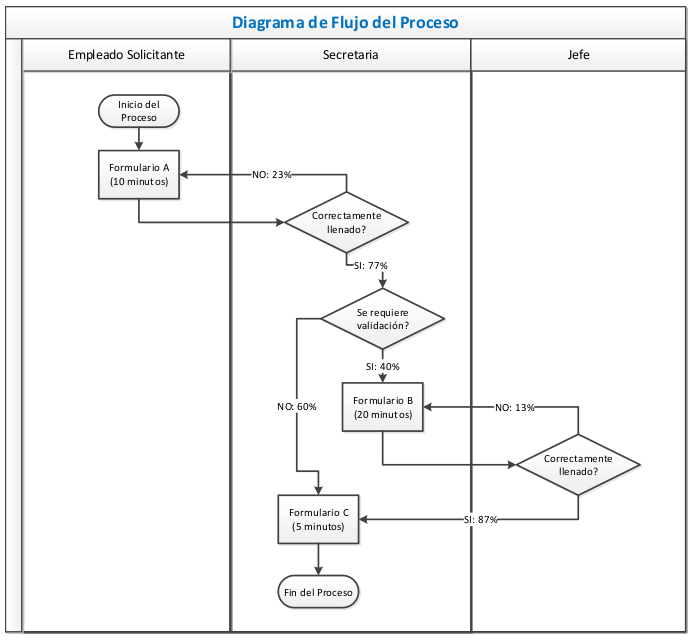
\includegraphics[width = 0.88\columnwidth]{figures/fig_burocracia.jpg}
\end{figure}

Con esto en mente, complete las siguientes actividades: 
\begin{enumerate}[label=\textbf{\alph*)}]
\item \textbf{[5 Puntos]} Modele el tr\'amite como una Cadena de Markov en Tiempo Discreto. 
\item \textbf{[5 Puntos]} Escriba, para cada estado, una ecuaci\'on cuya soluci\'on sea el tiempo esperado hasta el fin del proceso. 
\end{enumerate}

\QED

\end{problem}
\fullskip

% -----------------------------------------------------------------
\begin{problem}
Jos\'e es due\~no de una tienda al por menor que vende solamente un art\'iculo, el cual es importado de Estados Unidos. El tiempo que le toma a Jos\'e importar sus productos es de 6 d\'ias calendario, por lo que Jos\'e ha adoptado las siguientes reglas de negocio: 
\begin{itemize}
\item El inventario se mantiene siempre entre cero y cinco unidades. 
\item Cada lunes de ma\~nana, justo antes de abrir la tienda, Jos\'e observa el inventario y decide, en funci\'on del inventario, si importar 0, 2 o 4 unidades. Luego Jos\'e opera su tienda por seis d\'ias, hasta el s\'abado en la tarde. Finalmente, el s\'abado en la noche, justo despu\'es de cerrar la tienda, Jos\'e recibe las unidades que orden\'o el lunes de ma\~nana. 
\end{itemize}
Adicionalmente, Jos\'e ha estimado que la demanda te\'orica del art\'iculo, \ie el n\'umero de unidades que los clientes comprar\'ian si siempre hubiere inventario, es una variable aleatoria que obedece la siguiente distribuci\'on: 
\begin{table}[H]
\centering
\begin{tabular}{|c|c|c|c|c|c|c|}
\hline
$\boldsymbol{k}$ & 0 & 1 & 2 & 3 & 4 & 5 \\ \hline
$\boldsymbol{\Pr( D = k )}$ & 0.20 & 0.30 & 0.20 & 0.15 & 0.10 & 0.05 \\ \hline
\end{tabular}
\end{table}

Con esto en mente, modelaremos esta situaci\'on como un Proceso de Decisi\'on Markoviano donde los estados son el n\'umero de art\'iculos al comienzo de cada semana, \ie el lunes de ma\~nana justo antes de abrir la tienda. En particular: 
\begin{enumerate}[label=\textbf{\alph*)}]
\item \textbf{[3 Puntos]} Construya una tabla donde se muestren los estados en las filas y las acciones en las columnas. Luego indique las acciones disponibles en cada estado. 
\item \textbf{[12 Puntos]} Para cada estado, y para cada acci\'on disponible en ese estado, tabule las probabilidades de transici\'on. 
\end{enumerate}

\emph{Nota:} En este problema no he inclu\'ido una estructura de costos o recompensas con el prop\'osito de aligerar su carga de trabajo. 

\QED

\end{problem}
\fullskip

% -----------------------------------------------------------------
\begin{problem}
Un banco est\'a considerando abrir una nueva sucursal. Se estima que si se abre la sucursal los clientes arribar\'an de acuerdo a un proceso Poisson con tasa media de 60 por hora. Adem\'as, se conoce que el tiempo de servicio en ventanilla se puede modelar como una variable aleatoria exponencial con media de 3.5 minutos. 

Con esto en mente, complete las siguientes actividades: 
\begin{enumerate}[label=\textbf{\alph*)}]
\item \textbf{[1.5 Puntos]} Encuentre el n\'umero m\'inimo de cajeros requeridos para garantizar la estabilidad del sistema de colas. Este n\'umero ser\'a llamado $k_{min}$. 
\item \textbf{[7.5 Puntos]} Calcule las m\'etricas de desempe\~no $L_q$ y $W_q$ para el caso cuando se operan las ventanillas con $k_{min}$ cajeros, $k_{min} + 1$ cajeros, y $k_{min} + 3$ cajeros. 
\item \textbf{[1.5 Puntos]} Suponga ahora que los cajeros humanos son remplazados por cajero autom\'aticos. Como consecuencia, en este caso los tiempos de servicio pueden ser modelados como constantes iguales a 2.8 minutos. Encuentre el n\'umero m\'inimo de cajeros requeridos para garantizar la estabilidad del sistema de colas. Este n\'umero ser\'a llamado $n_{min}$. 
\item \textbf{[7.5 Puntos]} Recalcule las m\'etricas de desempe\~no $L_q$ y $W_q$ para el caso cuando se operan $n_{min}$ cajeros autom\'aticos, $n_{min} + 1$ cajeros autom\'aticos, y $n_{min} + 2$ cajeros autom\'aticos. 
\end{enumerate}

Para resolver el problema puede hacer uso del siguiente par de figuras: 
\begin{figure}[H]
\centering
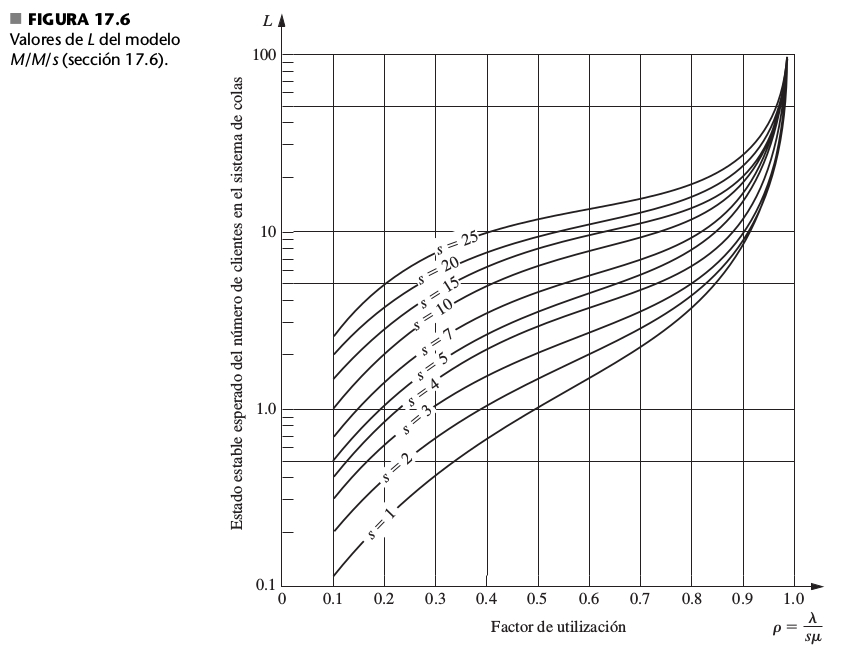
\includegraphics[width = 1.06\columnwidth]{figures/fig_metricas-MMS.jpg}
\end{figure}
\begin{figure}[H]
\centering
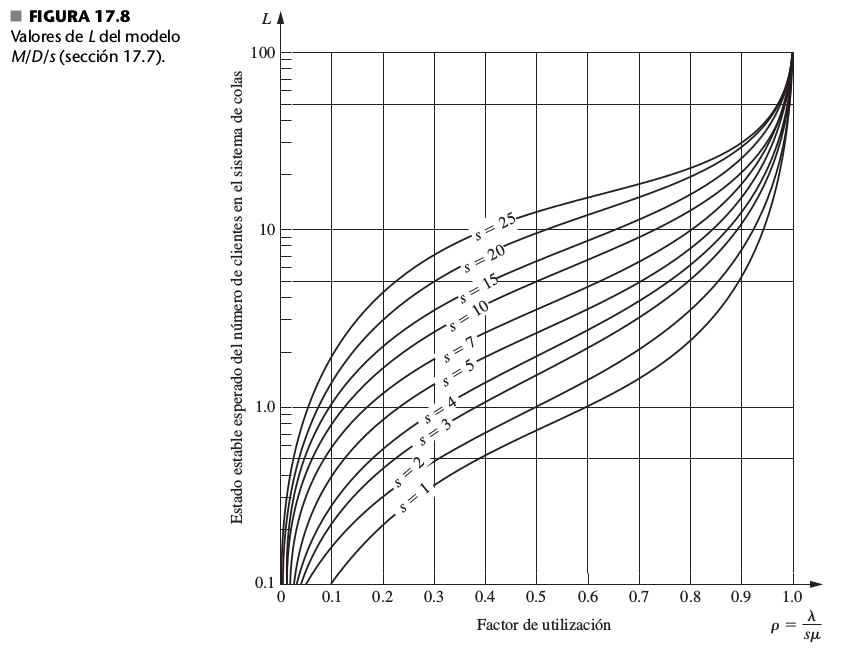
\includegraphics[width = 1.06\columnwidth]{figures/fig_metricas-MDS.jpg}
\end{figure}

\QED

\end{problem}
\fullskip

\end{document}
